\white{Fusion 360}
\chapterauthor{Connor Albers}
\section*{The Importance of Designing Before Building}  
\info{Connor Albers}{Fusion 360}{October 4, 2024}
Designing your robot before actually building it is important for any team, as it allows potential problems to be solved prior to construction, preventing wasted parts. It also enables teams to explore different ideas faster and more efficiently. For many teams, a simple drawing is all they need to get started building, but our team decided to go the digital route with computer-aided design (CAD). Using CAD allows our team to not only view our designs in 3D but also aids us in designing to scale, ensuring every piece fits just as it would in real life.

\section*{Options for CAD Software in VEX Robotics}  
When designing VEX robots specifically, there are many options, such as Onshape or Fusion 360. Both programs are popular within the VEX community and thus have large file folders containing 3D models of every official VEX part. These folders make it easy to import parts and design robots more efficiently, removing the need to download parts individually from the VEX website.

\section*{Advantages and Challenges of Using CAD}  
While these software platforms feature steep learning curves for new users, they offer many benefits. Importing parts manually means users can add new parts just as they are released on the VEX official website. Additionally, teams may import or create custom parts to fit their specific needs. These custom parts can then be laser-cut, CNC-machined, or 3D-printed to create components accurately.

\section*{Collaboration and File Exporting}  
Collaboration is another key advantage of these software platforms; both allow the user to add others to documents, promoting teamwork within the group. Additionally, these more generic CAD programs allow the user to export files in industry-standard formats, enabling the team to accurately simulate their robot in other programs.

\section*{Protobot: A User-Friendly Alternative}  
Another, more user-friendly option is a community project called Protobot. Protobot is software that allows users to create robots virtually using VEX parts. What’s special about this software is that it is designed specifically for VEX V5 robot construction, so every part is imported and ready to use. Combined with optimized part-collaging features, Protobot is the most user-friendly CAD program for designing VEX robots.

\section*{Drawbacks of Protobot}  
This accessibility does have its drawbacks. First, the parts catalog is not always up to date; new parts may take an extended period to be added to the program. Second, as of October 2024, the software does not support live file sharing, meaning the only way to share models is to download and send them via email or other mediums, making collaboration difficult. Finally, the software does not allow users to import or design custom parts, making it challenging for advanced teams to accurately construct their robots.

\section*{Why We Chose Fusion 360}  
With all this information in mind, our team decided to use Fusion 360 to design our future robots. Fusion 360 was the obvious choice for our team because many of our members already had experience using the program. Also, from what we had heard from other teams, Fusion was far more powerful than other programs, such as Onshape, due to it running locally on the user’s device rather than over the cloud. A final advantage of using a generic CAD program is that we planned on creating a virtual simulation, which would require standard files not supported in Protobot.

\important{Pre Douglas Coding (October 10, 2024)}
\chapterauthor{Ian Smith}
\info{Ian Smith}{Pre Douglas Coding}{October 10, 2024}
\section*{Coding in Robot Design}

Coding is a very critical part of robot design, especially when considering the most current mechanical design. Within the software, we will have to perform complex kinematics, graphic design, and dynamic programming within the C++ language. The coding of this bot started with an accurate LemLib setup for our bot.

%\begin{lstlisting}[language=C++, caption={LemLib Setup}, label={lst:lemlib_setup}]
%(insert code here)
%\end{lstlisting}

I wrote the basic controls for the pneumatics on a toggle and implemented expo drive. After a meeting with the drive team, a few concepts were discussed:
\begin{itemize}
    \item Displaying match status on the brain
    \item Displaying match status on the controller
    \item Custom controller layouts for both drivers
    \item Motor status during a match (color-coded on the brain)
    \item Chase proposed the idea of using both controllers (buddy controller), but switchable
\end{itemize}

Knowing that all the requested ideas were feasible within the hardware, I knew I could write a software solution to meet the design requirements. 

\subsection*{Switchable Controllers}
I first decided to tackle the switchable controllers as this seemed to be the most relevant feature. I created a class called \texttt{my\_controller} that contained public variables for each button and mapped control. Originally, I used the \texttt{int} variable type because the enumerated values within the \texttt{pros} namespace expand into small integers. However, this didn’t work, and I had to switch to the \texttt{pros::controller::E\_DIGITAL\_PRESSING} type. This correctly allowed button mapping on the controllers, varied by different instances of the class.

I declared the subsequent class and initialized the mapping for each user. Another instance, called \texttt{current}, had the currently selected controller class instance written to it. A function was created to determine which controller was current based on the last “give away” or “switch controller” button. 

There were a few issues overall, primarily due to the \texttt{get\_digital} functions only accepting special \texttt{pros} variable types for buttons, along with issues in passing controller objects by reference. However, overall, the implementation was quick and easy.

\subsection*{Motor Status Color Coding}
The next challenge I undertook was adding color coding for motor states based on temperature. I knew that motors cut out in increments, but I didn’t know the specifics. The general idea was that the motors would reduce their maximum power, and we could display this on the brain. 

For this, I referred to a VEX Forum post (\href{https://www.vexforum.com/t/v5-motor-temp-in-percent/52433}{https://www.vexforum.com/t/v5-motor-temp-in-percent/52433}) and used the response by \texttt{jpearman}. I set up circles on the V5 brain to coordinate with the eight motors on the robot, filling them with the appropriate color (green, yellow, or red) depending on motor state. Initially, I encountered arithmetic and color errors when trying to print to the brain.

\subsection*{Future Features}
The drivers are requesting a “Print to Controller” system for mid-match monitoring. I haven't implemented this yet due to time constraints. I also sketched out a few mock autonomous routines for LemLib, though I am still experiencing issues with my IMU and rotational PID. The autonomous routines are selected on an autonomous selection screen, which consists of boxes activated by a \texttt{when\_pressing()} function.

\section*{LemLib: An Overview and Implementation}  

LemLib is a student-developed, open-source library for VEX VRC that is feature-rich and easy to use \href{https://github.com/LemLib/LemLib}{(this is a link to the LemLib GitHub project)}. After successfully writing my own PID controller and beginning work on a pure pursuit algorithm, I realized that using a library would streamline the development of our autonomous routines—something I could have implemented from scratch but found more efficient through LemLib.  

In order to use LemLib, the process revolves around a few simple principles.  

\subsection*{Setting up LemLib}  
The first step was importing the LemLib depot from GitHub into my development environment.  
\begin{quote}
\textbf{Author's Note:} I am using Ubuntu 22.04 with the PROS extension over Visual Studio Code as my setup.  
\end{quote}

The LemLib documentation provides clear examples on how to import the library. In the PROS terminal, I executed the following commands:  

\begin{verbatim}
$ pros c add-depot LemLib https://raw.githubusercontent.com/LemLib/LemLib/depot/stable.json
$ pros c apply LemLib
\end{verbatim}

\subsection*{Initializing Motors and Sensors}  
After importing the library, the next step was to add the appropriate motors and motor groups. Since we are using an Inertial Measurement Unit (IMU) to measure the robot’s heading ($\theta$), we had to declare an instance of the IMU class. Initially, we encountered an issue with the IMU, as the heading value continuously decreased when the robot was stationary. To resolve this, we replaced the faulty IMU with the one from Capten’s Worlds robot.  

The next task was to initialize the sensors for odometry. Although we originally planned to use an odometry pod, we did not have enough space on our robot. As a substitute, we used the drivetrain's motor encoders (IMEs), which are less accurate but still functional for tracking. Afterward, I created an instance of the \verb|sensors| class, passing in the necessary configuration parameters.  

We also utilize the controller curves provided by LemLib, as discussed in Chapter . All this information is combined to create an instance of the \verb|drivetrain| class.  

\subsection*{Initializing the Chassis}  
Within the initialization loop, we had to declare:  

\begin{verbatim}
chassis.initialize();
\end{verbatim}

At this point, our code was ready to be tuned.  

\paragraph{Note:}  
For months, we faced issues with the chassis not initializing properly. After countless hours of troubleshooting and communicating with the developers, we finally identified the problem. Our code mistakenly included:  

\begin{verbatim}
void initalize() {}
\end{verbatim}

The correct code should have been:  

\begin{verbatim}
void initialize() {}
\end{verbatim}

Did you spot the difference? That missing letter in the function name caused all our issues!  

\subsection*{Tuning the Autonomous Functions}  
When tuning the autonomous routines, we began with the angular PID (Proportional-Integral-Derivative) controller. We started with a small proportional gain ($k_P$) and gradually increased the derivative gain ($k_D$) until the robot stopped with high accuracy while maintaining maximum speed into a stop.  

In this scenario, tuning the integral gain ($k_I$) was unnecessary since the robot did not need to maintain specific positions—such as holding an arm steady. The same procedure was followed for the lateral PID controller, ensuring the robot was fully tuned.  

\subsection*{Implementing Pure Pursuit Paths}  
With our PID tuning complete, the next step is to input the paths from our concepts into LemLib’s pure pursuit algorithm. We plan to complete this task in the days leading up to the Douglas competition.  

\subsection*{Conclusion}  
Our LemLib implementation is now fully documented and explained, providing a solid foundation for our robot’s autonomous capabilities. The skeleton project ensures that all aspects are correctly configured and ready for testing.



\white{Robot V1 (October 16, 2024)}
\chapterauthor{Caleb Bachmeier}
\info{Caleb Bachmeier}{Robot V1}{October 16, 2024}
\textbf{Goal}: This chapter will explain our first robot
\section*{Robot V1}
Below are complete pictures of our first robot in Fusion 360:
%Pictures of the robot in fusion 360
\subsection*{Drivetrain}
Drivetrain stats:
\begin{itemize}
    \item 66 Watts
    \item 480 RPM
    \item 14.75"
    \item Peak velocity is 82/inches per second
\end{itemize}
\begin{figure}[hbt!] % Use [hbt!] to place the figures on the same page
    \begin{minipage}{.5\textwidth}
        \centering
        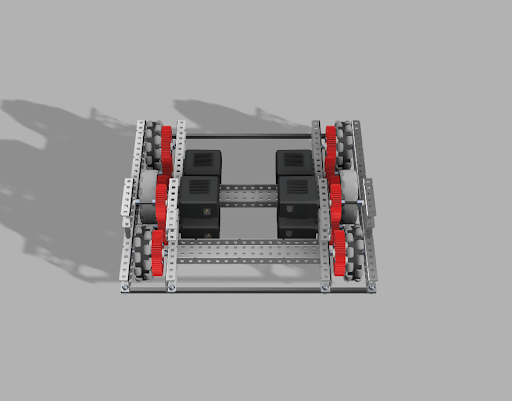
\includegraphics[width=.8\linewidth]{images/Frontdown-V1-Drivetrain.png}
        \caption{Front view}
        \label{fig:frontdown}
    \end{minipage}
    \begin{minipage}{.5\textwidth}
        \centering
        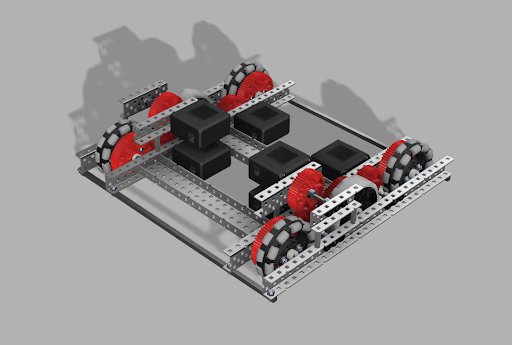
\includegraphics[width=.8\linewidth]{images/Iso-V1-Drivetrain.png}
        \caption{Isometric view}
        \label{fig:iso}
    \end{minipage}
    \begin{minipage}{.5\textwidth}
        \centering
        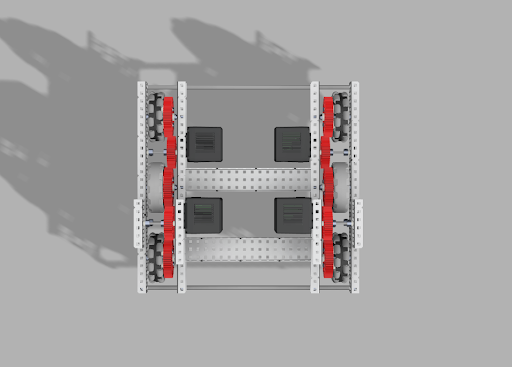
\includegraphics[width=.8\linewidth]{images/Topdown-V1-Drivetrain.png}
        \caption{Top view}
        \label{fig:topdown}
    \end{minipage}
    \begin{minipage}{.5\textwidth}
        \centering
        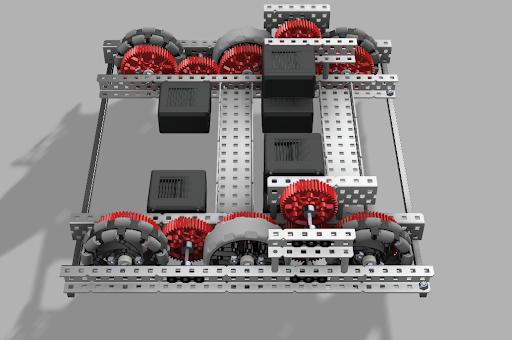
\includegraphics[width=.8\linewidth]{images/Sidedown-V1-Drivetrain.png}
        \caption{Side view}
        \label{fig:sidedown}
    \end{minipage}
\end{figure}

Above are our finished drivetrain CAD images.
\subsection*{Clamp}
Clamp stats:
\begin{itemize}
    \item Uses two, 12 pound, pneumatic pistons 
    \item Clamps the corner of 
\end{itemize}
\begin{figure}[h!] % Use [hbt!] to place the figures on the same page
    \begin{minipage}{.55\textwidth}
        \centering
        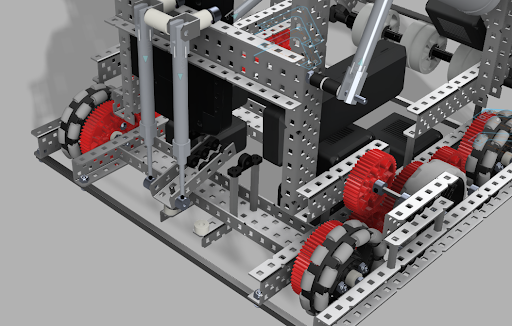
\includegraphics[width=1\linewidth]{images/Iso-Clamp-V1.png}
        \caption{Isometric View}
        \label{fig:iso}
    \end{minipage}
    \begin{minipage}{.55\textwidth}
        \centering
        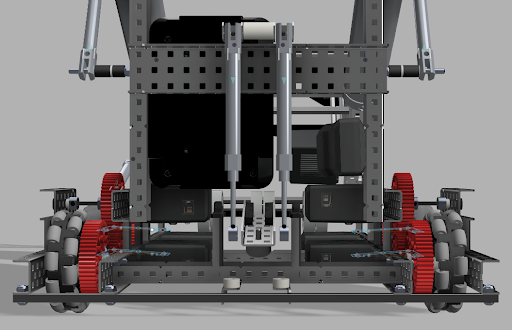
\includegraphics[width=1\linewidth]{images/Front-Clamp-V1.png}
        \caption{Front View}
        \label{fig:front}
    \end{minipage}
    \begin{minipage}{.55\textwidth}
        \centering
        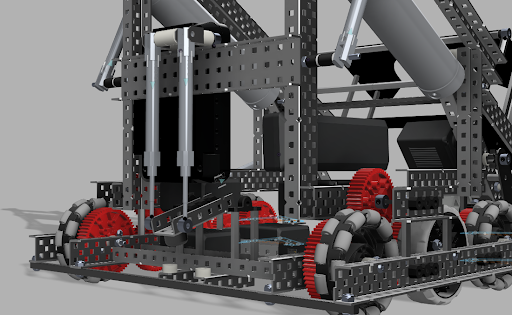
\includegraphics[width=1\linewidth]{images/Side-Clamp-V1.png}
        \caption{Side View}
        \label{fig:side}
    \end{minipage}
    \begin{minipage}{.55\textwidth}
        \centering
        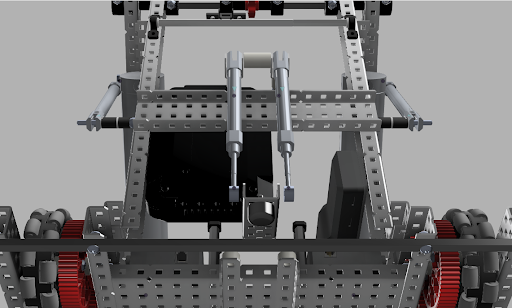
\includegraphics[width=1\linewidth]{images/Bottom-Clamp-V1.png}
        \caption{Bottom View}
        \label{fig:bottom}
    \end{minipage}
\end{figure}

Above are pictures of our Clamp in Fusion 360
\subsection*{Hook Intake}
Hook Intake stats:
\begin{itemize}
    \item Uses 22 watts of power
    \item Uses acetal hooks to grab rings and place them on Mobile Goals
\end{itemize}

\subsection*{Robot V1}
This is our entire first robot or Robot V1. Below are Fusion 360 pictures of the entire thing, the only thing it is missing is the chain on the Hook Intake.
